\documentclass[11pt]{article}

\usepackage{amsfonts,amsmath,amssymb,amsthm}
\usepackage[normalem]{ulem} % temporary for strikeout math
\usepackage{enumerate}
\usepackage[shortlabels,inline]{enumitem}
\usepackage{wrapfig}

\usepackage[lined,noend]{algorithm2e}
\usepackage{tabularx}
\usepackage{colortbl}
\usepackage{adjustbox}
\DontPrintSemicolon

\PassOptionsToPackage{hyphens}{url}
\usepackage{fullpage}
\usepackage{hyperref}
\usepackage{xcolor}
\usepackage{xifthen}
\usepackage{placeins}
\usepackage{pifont}
\usepackage{multirow}
\usepackage{tikz}
\usepackage{pgfplots}
\usepackage[framemethod=tikz]{mdframed} % and thus tikz
\usepackage[font=small]{caption}

\usepackage{authblk}

% footnotes in table and tabular
\usepackage{footnote}
\makesavenoteenv{tabular}
\makesavenoteenv{table}
\makesavenoteenv{figure}

\usepackage{stmaryrd} % fancy double square brackets

\setcounter{tocdepth}{2} % Override LLNCS

% ==== Hydra Macros ====

% NOTE: New macro file; please copy and keep organized macros from
% macros_old.tex as needed.  Hopefully, this will result in tidier
% macros file.
%
% Index:
% - Misc
% - General
% - Theorem Environments
% - Multisignatures
% - Transactions
% - State Machines
% - Head Protocol
% - On-Chain Verification
% - Algorithms
% - Merkle-Patricia Trees

% === engineering ===
\newcommand{\undefined}{\mathrm{undef}}


% === Misc ===

\newcommand{\algoskip}{\vspace{4pt}}

\newcommand{\ignore}[1]{}

\newcommand{\TODO}[1]{
  \if\relax\detokenize{#1}\relax
    \textcolor{red}{TODO}
  \else
    \textcolor{red}{ {#1}}
  \fi
}

\newcommand{\fail}{\mbox{fail}}

% from https://www.overleaf.com/latex/examples/simple-stylish-box-design/stzmmcshxdng
\definecolor{main}{HTML}{5989cf}    % setting main color to be used
\definecolor{sub}{HTML}{cde4ff}     % setting sub color to be used
\newtcolorbox{boxM}{
    fontupper = \color{white},
    rounded corners,
    arc = 6pt,
    colback = main!80, 
    colframe = main, 
    boxrule = 0pt, 
    bottomrule = 4.5pt,
    enhanced,
    fuzzy shadow = {0pt}{-3pt}{-0.5pt}{0.5pt}{black!35}
}

% In figures, this makes algorithms work with option [H] despite
% double-column format
% https://tex.stackexchange.com/questions/82271/multiple-algorithm2e-algorithms-in-two-column-documents
\makeatletter
\newcommand{\removelatexerror}{\let\@latex@error\@gobble}
\makeatother

\newcommand{\md}{\textsf{-}}

\newcommand{\fst}[1]{#1^{\text{st}}}
\newcommand{\snd}[1]{#1^{\text{nd}}}
\newcommand{\trd}[1]{#1^{\text{rd}}}
\newcommand{\ith}[1]{#1^{\text{th}}}

\newcommand{\eps}{\varepsilon}
\newcommand{\mc}{\mathcal}

\DeclareMathOperator*{\argmax}{arg\,max}
\DeclareMathOperator*{\argmin}{arg\,min}


% === General ===
\newcommand{\ol}[1]{\overline{#1}}

\newcommand{\true}{\mathtt{true}}
\newcommand{\false}{\mathtt{false}}

\newcommand{\spara}{k}

\newcommand{\nop}{n}
\newcommand{\party}{\mathsf p}
\newcommand{\parties}{\mathcal{P}}

\newcommand{\adv}{\ensuremath{\mathcal{A}}}
\newcommand{\att}{\adv}
\newcommand{\advLive}{\ensuremath{\mathcal{A}}_{\mathsf L}}

\newcommand{\propName}{\textsc}

\newcommand{\hout}[1]{h_{\mathsf{out},#1}}
\newcommand{\hrest}{h_{\mathsf{rest}}}

\newcommand{\es}{\eps}

\newcommand{\hash}{\mathsf{hash}}
\newcommand{\bytes}{\mathsf{bytes}}


% === Theorem Environments ===

\newtheoremstyle{putaneffinperiod}% name of the style to be used
  {\topsep}% measure of space to leave above the theorem. E.g.: 3pt
  {\topsep}% measure of space to leave below the theorem. E.g.: 3pt
  {\itshape}% name of font to use in the body of the theorem
  {0pt}% measure of space to indent
  {\bfseries}% name of head font
  {.}% punctuation between head and body
  {1em}% space after theorem head; " " = normal interword space
  {\thmname{#1}\thmnumber{ #2}\thmnote{ (#3)}}
\theoremstyle{putaneffinperiod}

\newtheorem{theorem}{Theorem}
% \numberwithin{theorem}{chapter}
\newtheorem{lemma}[theorem]{Lemma}
\newtheorem{corollary}[theorem]{Corollary}
\newtheorem{proposition}[theorem]{Proposition}
\newtheorem{claim}[theorem]{Claim}
\newtheorem{definition}{Definition}
% \numberwithin{definition}{chapter}
\newtheorem{invariant}{Invariant}
\newtheorem{axiom}[theorem]{Axiom}
\newtheorem{postulate}{Postulate}
\theoremstyle{definition}
\newtheorem{example}{Example}
\newtheorem{construction}{Construction}


% === Transactions ===

\newcommand{\tyBool}{\mathbb{B}}
\newcommand{\tyNatural}{\mathbb{N}}
\newcommand{\tyInteger}{\mathbb{Z}}
\newcommand{\tyData}{\mathsf{Data}}
\newcommand{\tyBytes}{\mathbb{H}}

\newcommand{\datum}{\delta} % a datum
\newcommand{\redeemer}{\rho} % a redeemer

\newcommand{\txContext}{\gamma} % validation context
\newcommand{\tyContext}{\Gamma} % type of contexts

\newcommand{\val}{\mathsf{val}} % a value
\newcommand{\tyValue}{\mathsf{Val}} % type of values

\newcommand{\tx}{\mathrm{tx}}
\newcommand{\txA}{\mathrm{txA}}
\newcommand{\txB}{\mathrm{txB}}
\newcommand{\validTx}{\mathsf{valid\md{}tx}}
\newcommand{\applytx}{\circ}
\newcommand{\Reach}{\mathsf{Reach}}

\newcommand{\txTx}{\mathit{tx}}			% transaction value
\newcommand{\txTxTy}{\mathit{Tx}}		% transaction type
\newcommand{\txCIdTy}{\mathit{CId}}		% currency identifier type
\newcommand{\txTokenTy}{\mathit{Token}}	        % currency token type
\newcommand{\txKeys}{\kappa} % (public) keys signing the tx
\newcommand{\tyKeys}{\mathcal{K}^*} % type of keys
\newcommand{\txOutRef}{\mathsf{out\md{}ref}}
\newcommand{\txInputs}{\mathcal{I}} % set of inputs
\newcommand{\tyInputs}{\mathcal{I}^*} % type of input sets
\newcommand{\txOutputs}{\mathcal{O}} % list of outputs
\newcommand{\tyOutputs}{\mathcal{O}^{\underline{*}}} % type of output lists
\newcommand{\txMint}{\mathsf{mint}} % minted value
\newcommand{\txID}{\mathit{txID}}
\newcommand{\ID}{\mathsf{ID}}
\newcommand{\txIdx}{\mathit{txIdx}}
\newcommand{\txR}{r}
\newcommand{\txRmin}{r_{\mathsf{min}}}
\newcommand{\txRmax}{r_{\mathsf{max}}}

\newcommand{\txIpend}{i_{\mathsf{pend}}}
\newcommand{\txIpendSet}{I_{\mathsf{pend}}}

\newcommand{\Tset}{T}
\newcommand{\Uset}{U}
\newcommand{\Uinit}{\Uset_{0}}
\newcommand{\Ufinal}{\Uset_{\mathsf{final}}}

\newcommand{\recordUTxO}{\mathsf{recordUTxO}}

% === Multisignatures ===

\newcommand{\ms}{\mathsf{MS}}

\newcommand{\msSetup}{\mathsf{MS\md{}Setup}}
\newcommand{\msKeyGen}{\mathsf{MS\md{}KG}}
\newcommand{\msSign}{\mathsf{MS\md{}Sign}}
\newcommand{\msVfy}{\mathsf{MS\md{}Verify}}
\newcommand{\msComb}{\mathsf{MS\md{}ASig}}
\newcommand{\msCombVK}{\mathsf{MS\md{}AVK}}
\newcommand{\msCombVfy}{\mathsf{MS\md{}AVerify}}

\newcommand{\msParams}{\Pi}
\newcommand{\msSig}{\sigma}
\newcommand{\msSigL}{\Sigma}
\newcommand{\msCSig}{\tilde\sigma}
\newcommand{\msVK}{k^{ver}}
\newcommand{\msCVK}{\tilde{k}}
\newcommand{\msVKL}{\mathcal{V}}
\newcommand{\msSK}{k^{sig}}
\newcommand{\msMsg}{m}

\newcommand{\initial}[1]{\dot{#1}}
%\newcommand{\chain}[1]{\dot{#1}}
\newcommand{\sVK}{k_{\pu}}
\newcommand{\sVKI}[1]{k_{#1,\pu}}
\newcommand{\sVKII}[1]{\initial{k}_{#1,\pu}}
\newcommand{\sSK}{k_{\pr}}
\newcommand{\sSKI}[1]{k_{#1,\pr}}
\newcommand{\sSKII}[1]{\initial{k}_{#1,\pr}}

% === State Machines ===

\newcommand{\cemS}{S_{\textsc{cem}}}
\newcommand{\cemI}{I_{\textsc{cem}}}
\newcommand{\cemIn}{i_{\textsc{cem}}}
\newcommand{\cemOut}{o_{\textsc{cem}}}
\newcommand{\cemValidator}{\nu_{\textsc{cem}}}
\newcommand{\cemDatum}{\datum_{\textsc{cem}}}
\newcommand{\cemRedeemer}{\redeemer_{\textsc{cem}}}
\newcommand{\cemFinal}{\mathit{final}_{\textsc{cem}}}
\newcommand{\cemStep}{\mathit{step}_{\textsc{cem}}}
\newcommand{\cemStepRel}[4]{{#1}\overset{#2}\longrightarrow(#3, #4)}
\newcommand{\cemTxCon}{\tx^\equiv}

\newcommand{\cid}{\mathsf{cid}} % head id / currency id

\newcommand{\st}{\mathsf{ST}}
\newcommand{\pt}{\mathsf{PT}}

% == Transactions ==

\newcommand{\mtxInit}{\textit{init}}
\newcommand{\mtxCom}{\textit{commit}}
\newcommand{\mtxCommit}{\textit{commit}}
\newcommand{\mtxCCom}{\textit{collectCom}}
\newcommand{\mtxCollect}{\textit{collectCom}}
\newcommand{\mtxIncrement}{\textit{increment}}
\newcommand{\mtxDecrement}{\textit{decrement}}
\newcommand{\mtxAbort}{\textit{abort}}
\newcommand{\mtxClose}{\textit{close}}
\newcommand{\mtxContest}{\textit{contest}}
\newcommand{\mtxFinalize}{\textit{finalize}}
\newcommand{\mtxFanout}{\textit{fanout}}
\newcommand{\mtxSplit}{\textit{split}}
\newcommand{\mtxCSN}{\textit{collectSN}}
\newcommand{\mtxCHT}{\textit{collectHT}}
\newcommand{\mtxSN}{\textit{SN}}
\newcommand{\mtxHT}{\textit{HT}}

% == States ==

\newcommand{\stInitial}{\mathsf{initial}}
\newcommand{\stOpen}{\mathsf{open}}
\newcommand{\stClosed}{\mathsf{closed}}
\newcommand{\stSnap}{\mathsf{newestSN}}
\newcommand{\stFinal}{\mathsf{final}}

\newcommand{\hMT}{h_{\mathsf{MT}}}
\newcommand{\piMT}{\pi_{\mathsf{MT}}}
\newcommand{\cPer}{T}
\newcommand{\Tfinal}{T_{\mathsf{final}}}
\newcommand{\Tsnapshot}{T_{\mathsf{newestSN}}}
\newcommand{\contesters}{\mathcal C}


% == Inputs ==

\newcommand{\stCollect}{\mathsf{collect}}
\newcommand{\stClose}{\mathsf{close}}
\newcommand{\stContest}{\mathsf{contest}}
\newcommand{\stFanout}{\mathsf{fanout}}
\newcommand{\stAbort}{\mathsf{abort}}


% == Validators ==

\newcommand{\muHead}{\mu_\mathsf{head}}
\newcommand{\nuHead}{\nu_\mathsf{head}}
\newcommand{\nuInitial}{\nu_\mathsf{initial}}
\newcommand{\nuCommit}{\nu_\mathsf{commit}}
\newcommand{\nuSnap}{\nu_\mathsf{SN}}
\newcommand{\nuNewname}{\nu_\mathsf{newestSN}}
\newcommand{\nuHang}{\nu_\mathsf{HT}}
\newcommand{\nuFinal}{\nu_\mathsf{final}}


% === Head Protocol ===

% == Algorithms ==

\newcommand{\HP}{\mathsf{HP}}
\newcommand{\hpSetup}{\mathsf{Setup}}
\newcommand{\hpKG}{\mathsf{KeyGen}}
\newcommand{\hpAgg}{\mathsf{Agg}}
\newcommand{\hpProt}{\mathsf{Prot}}


% == Protocol ==

\newcommand{\hpInit}{\mathtt{init}}
\newcommand{\hpNew}{\mathtt{new}}
\newcommand{\hpSeen}{\mathtt{seen}}
\newcommand{\hpConf}{\mathtt{conf}}
\newcommand{\hpClose}{\mathtt{close}}
\newcommand{\hpCont}{\mathtt{cont}}
\newcommand{\hpFO}{\mathtt{fanOut}}

\ignore{
\newcommand{\obj}{\Omega}

\newcommand{\certreq}{\ensuremath{\mathtt{sigReq}}}
\newcommand{\certack}{\ensuremath{\mathtt{sigAck}}}
\newcommand{\certconf}{\ensuremath{\mathtt{sigConf}}}

\newcommand{\abortreq}{\ensuremath{\mathsf{abortReq}}}

\newcommand{\init}{\mathbf{Init}}
\newcommand{\gencert}{\mathbf{GenCert}}

\newcommand{\txobj}{\mathsf{txo}}
\newcommand{\genobj}{\mathsf{obj}}
\newcommand{\genset}{\mathsf{ObjSet}}
\newcommand{\gentxobj}{\mathsf{GenTxObj}}
\newcommand{\stateobj}{\ensuremath{u}}
\newcommand{\ack}{\mathsf{ack}}
}

% == Variables ==
\newcommand{\pu}{\mathsf{ver}}
\newcommand{\pr}{\mathsf{sig}}


\newcommand{\hpParams}{\Sigma}
\newcommand{\hpPu}{K_{\pu}}
\newcommand{\hpPuv}{\underline{K}_\pu}
\newcommand{\hpPui}[1]{K_{\pu,#1}}
\newcommand{\hpPr}{K_{\pr}}
\newcommand{\hpPri}[1]{K_{\pr,#1}}

\newcommand{\hpAK}{\tilde{k}_{\mathsf{H}}} % Aggregated hydra key
\newcommand{\hppuv}{\underline{k}_C} % List of cardano keys
\newcommand{\keyHash}{k^{\#}} % Some verification key hash

\newcommand{\hpPuvInit}{\initial{\underline{K}}_\pu}

\newcommand{\hpAKchain}{\hpAK^{\mathsf{chain}}}
\newcommand{\hpAKinit}{\hpAK^{\mathsf{setup}}}

%\newcommand{\initial}{\mathsf{init}}
\newcommand{\daPuII}[1]{\initial{K}_{#1,\pu}}
\newcommand{\daPrII}[1]{\initial{K}_{#1,\pr}}
%\newcommand{\sVKI}{\mathsf{vk}^{\initial}}
%\newcommand{\sSKI}{\mathsf{sk}^{\initial}}

\newcommand{\hppuvinit}{\initial{\underline{k}}_\pu}


\newcommand{\hats}{\hat s}
\newcommand{\bars}{\overline s}
\newcommand{\hatmU}{\hat {\mathcal U}}
\newcommand{\barmU}{\overline {\mathcal U}}
\newcommand{\mL}{{\mathcal L}}
\newcommand{\hatmL}{\hat {\mathcal L}}
\newcommand{\barmL}{\overline {\mathcal L}}
\newcommand{\mT}{{\mathcal T}}
\newcommand{\hatmT}{\hat {\mathcal T}}
\newcommand{\barmT}{\overline {\mathcal T}}
\newcommand{\hatmDT}{\Delta\hat {\mathcal T}}
\newcommand{\hatmR}{\hat {\mathcal R}}
\newcommand{\mH}{{\mathcal H}}

\newcommand{\TR}{T_{\mathsf R}}
\newcommand{\tTR}{\tilde T_{\mathsf R}}
\newcommand{\tR}{\tilde R}

\newcommand{\hpSigs}{S}

\newcommand{\txo}{\mathsf{tx}}


% == Commands ==

\newcommand{\hpRG}{\mathtt{req}}
\newcommand{\hpAG}{\mathtt{ack}}
\newcommand{\hpCG}{\mathtt{conf}}

\newcommand{\hpRT}{\mathtt{reqTx}}
\newcommand{\hpAT}{\mathtt{ackTx}}
\newcommand{\hpCT}{\mathtt{confTx}}

\newcommand{\hpNS}{\mathtt{newSn}}
\newcommand{\hpRS}{\mathtt{reqSn}}
\newcommand{\hpAS}{\mathtt{ackSn}}
\newcommand{\hpCS}{\mathtt{confSn}}


% == Functions ==

\newcommand{\Txo}{\mathsf{txObj}}
\newcommand{\Sno}{\mathsf{snObj}}
\newcommand{\ApplyMax}{\mathsf{uApplyMax}}

\newcommand{\hpLdr}{\mathsf{leader}}
\newcommand{\hpMT}{\mathsf{maxTxos}}

\newcommand{\conf}{\mathsf{conflict}}
\newcommand{\confTx}{\mathsf{conflict\md{}tx}}

% serialisation
\newcommand{\bits}{\mathsf{bits}}

% == Projectors ==

\newcommand{\hpProj}{_{\downarrow (\tx,\msCSig)}}
\newcommand{\hpProjT}{_{\downarrow (\tx)}}
\newcommand{\hpProjH}{_{\downarrow (\hash)}}
\newcommand{\hpProjSig}{_{\downarrow (\msCSig)}}
\newcommand{\hpProjHs}{_{\downarrow (\hash,\msCSig)}}
\newcommand{\hpProjSo}{_{\downarrow (s,\outputset)}}
\newcommand{\hpProjSos}{_{\downarrow (s,\outputset,\msCSig)}}

\renewcommand{\hpProj}{^{\downarrow (\tx,\msCSig)}}
\renewcommand{\hpProjT}{^{\downarrow (\tx)}}
\renewcommand{\hpProjH}{^{\downarrow (\hash)}}
\renewcommand{\hpProjSig}{^{\downarrow (\msCSig)}}
\renewcommand{\hpProjHs}{^{\downarrow (\hash,\msCSig)}}
\renewcommand{\hpProjSo}{^{\downarrow (s,\outputset)}}
\renewcommand{\hpProjSos}{^{\downarrow (s,\outputset,\msCSig)}}


% == Security ==

\newcommand{\Ttilde}{\tilde{T}}
\newcommand{\That}{\hat{T}}
\newcommand{\Tbar}{\overline{T}}
\renewcommand{\Ttilde}{\tilde{S}}
\renewcommand{\That}{\hat{S}}
\renewcommand{\Tbar}{\overline{C}}

\newcommand{\TxNewAll}{{\cal N}}

\newcommand{\Hcont}{H_{\mathsf{cont}}}
\newcommand{\honest}{\mathcal H}
\newcommand{\contSet}{\mathcal C}
\newcommand{\Cchain}{C_{\mathsf{chain}}}
\newcommand{\USN}[1]{\mathrm{SN}_{#1}}
\newcommand{\setSN}[1]{\tilde T_{#1}}
\newcommand{\curSN}[1]{\mathrm{SN}_{\mathsf{cur},#1}}

\newcommand{\INV}[1]{\mathsf{INV}_{#1}}

\newcommand{\atti}[1]{^{(#1)}}

% === Mediator Protocol ===
\newcommand{\gcClientNewHead}{\mathtt{clientNewHead}}
\newcommand{\gcClientTx}{\mathtt{clientTx}}
\newcommand{\gcClientClose}{\mathtt{closeTx}}
\newcommand{\gcChainInitial}{\mathtt{initialTx}}
\newcommand{\gcChainCollectCom}{\mathtt{collectComTx}}
\newcommand{\gcChainClose}{\mathtt{closeTx}}
\newcommand{\gcChainContest}{\mathtt{contestTx}}
\newcommand{\gcChainFanout}{\mathtt{fanoutTx}}
\newcommand{\gcChainAbort}{\mathtt{abortTx}}
\newcommand{\gcChainCommit}{\mathtt{commitTx}}
\newcommand{\gcChainInitialTO}{\mathtt{chainInitialTimeOut}}
\newcommand{\gcChainClosedTO}{\mathtt{chainClosedTimeOut}}

\newcommand{\gcChainRef}{\mathsf{chain}}
\newcommand{\gcClientRef}{\mathsf{client}}
\newcommand{\gcHeadRef}{\mathsf{head}}
\newcommand{\gcChainPost}{\mathsf{postTx}}
\newcommand{\gcUTXOset}{\mathsf{UTxOs}}
\SetKw{Call}{call}


% === On-Chain Verification ===

% == Algorithms and Oracles ==

\newcommand{\ocvInitial}{\mathsf{Initial}}
\newcommand{\ocvFinalize}{\mathsf{Finalize}}
\newcommand{\ocvClose}{\mathsf{Close}}
\newcommand{\ocvContest}{\mathsf{Contest}}
\newcommand{\ocvFinal}{\mathsf{Final}}

\newcommand{\ocvIncrement}{\mathsf{Increment}}
\newcommand{\ocvDecrement}{\mathsf{Decrement}}

\newcommand{\ocvSnapshot}{\mathsf{Snapshot}}
\newcommand{\ocvValidSnap}{\mathsf{ValidSN}}
\newcommand{\ocvValidHang}{\mathsf{ValidHT}}

\newcommand{\ocvClaim}{\mathsf{Claim}}
\newcommand{\ocvAllocate}{\mathsf{Allocate}}
\newcommand{\ocvFanout}{\mathsf{Fanout}}

\SetKwFor{OocvInitial}{$\ocvInitial$}{}{enddo}
\SetKwFor{OocvFinalize}{$\ocvFinalize$}{}{enddo}
\SetKwFor{OocvClose}{$\ocvClose$}{}{enddo}
\SetKwFor{OocvContest}{$\ocvContest$}{}{enddo}
\SetKwFor{OocvFinal}{$\ocvFinal$}{}{enddo}

\SetKwFor{OocvClaim}{$\ocvClaim$}{}{enddo}
\SetKwFor{OocvAllocate}{$\ocvAllocate$}{}{enddo}
\SetKwFor{OocvFanout}{$\ocvFanout$}{}{enddo}


% == Variables ==

\newcommand{\hInit}{\hash_{\mathsf{init}}}
\newcommand{\imax}{i_{\mathsf{max}}}
\newcommand{\symFinal}{\mathtt{final}}


% == Functions ==

\newcommand{\applicable}{\mathsf{applicable}}


% === Algorithms ===

% == Misc ==

% \setlength{\algomargin}{0em}


% == Boxes ==

\newenvironment{algobox}[1]%
{
  \begin{tabularx}{\textwidth}{X c X}
    \hline
    \rowcolor{gray!20} 
    & \textbf{#1} & \\
    \hline
  \end{tabularx}
  
  \vspace{-1.5em}

  \begin{center}
}
{
  \end{center}

  \vspace{-1.5em}

  \begin{tabularx}{\textwidth}{X c X}
    \hline
  \end{tabularx}

  \vspace{0.5em}
}

\newenvironment{walgo}[1]%
{
  \begin{minipage}{#1\linewidth}
    \begingroup
    \removelatexerror% Nullify \@latex@error
    \begin{algorithm}[H]  
}
{
    \end{algorithm}
    \endgroup
  \end{minipage}
}


% == Keywords ==

\SetKwFor{Check}{check}{}{enddo}


% == DA Game ==

%\newcommand{\algoskip}{\vspace{2pt}}

\SetKwIF{If}{ElseIf}{Else}{if}{}{else if}{else}{end if}
\SetKwFor{For}{for}{}{end for}

\SetKwFor{On}{on}{}{enddo}
\SetKwFor{Function}{function}{}{enddo}
\SetKwFor{PFunction}{public function}{}{enddo}
\SetKw{Out}{output}
\SetKw{Req}{require}
\SetKwFor{ForA}{for all}{}{enddo}
\SetKwFor{Wait}{wait}{}{enddo}
\SetKw{KwWait}{wait} % without body
\SetKw{IfI}{if}
\SetKw{ThenI}{then}
\SetKw{ElsI}{else}
\SetKw{FiI}{fi}

\newcommand{\daPID}{\mathsf{ID}}

\newcommand{\daGlobal}{\Sigma}
\newcommand{\daPu}{K_{\pu}}
\newcommand{\daPuV}{\overline K_{\pu}}
\newcommand{\daPuI}[1]{K_{#1,\pu}}
\newcommand{\daPr}{K_{\pr}}
\newcommand{\daPrI}[1]{K_{#1,\pr}}

\newcommand{\daCInit}{\mathtt{init}}
\newcommand{\daCNew}{\mathtt{new}}
\newcommand{\daCSeen}{\mathtt{seen}}
\newcommand{\daCConf}{\mathtt{conf}}
\newcommand{\daCCert}{\mathtt{cert}}
\newcommand{\daCComp}{\mathtt{comp}}

\SetKw{New}{new}
\SetKw{KwOn}{on}
\SetKw{Send}{send}
\SetKw{Multi}{multicast}
\SetKw{PostTx}{postTx}
\newcommand{\Store}{\mathsf{store}}
\newcommand{\Sign}{\mathsf{sign}}
\newcommand{\Combine}{\mathsf{sigCombine}}
\newcommand{\Verify}{\mathsf{SigVerify}}
\newcommand{\Complete}{\mathsf{Complete}}

\newcommand{\hyPu}{\msCVK}
\newcommand{\hyPr}{\msSK}


% === Merkle-Patricia Trees ===

% == Misc ==

\newcommand{\MPTalph}{A}

% == Algorithms ==

\newcommand{\MPTInit}{\mathsf{MPT\md{}Init}}
\newcommand{\MPTHash}{\mathsf{MPT\md{}Hash}}
\newcommand{\MPTMemb}{\mathsf{MPT\md{}Memb}}

\newcommand{\MPTBuild}{\mathsf{MPT\md{}Build}}
\newcommand{\MPTPath}{\mathsf{MPT\md{}Path}}


% == Hash Computations ==

\newcommand{\MPTverMemb}{\mathsf{MPT\md{}VfyMemb}}
\newcommand{\MPTcompRA}{\mathsf{MPT\md{}CompRA}}
\newcommand{\MPTcompSpl}{\mathsf{MPT\md{}CompSpl}}


% == Helpers ==

\newcommand{\CP}{\mathsf{CP}}
\newcommand{\RP}{\mathsf{RP}}
\newcommand{\Proj}{\mathsf{Proj}}
\newcommand{\Sum}{\mathsf{Sum}}
\newcommand{\Size}{\mathsf{Size}}
\newcommand{\First}{\mathsf{First}}


% == Oracles ==

\SetKwFor{MPTAInit}{\sf MPT-Init}{}{enddo}

\SetKwBlock{MPTAHash}{\sf MPT-Hash}{enddo}
\SetKwFor{MPTAMemb}{\sf MPT-Memb}{}{enddo}

\SetKwFor{MPTABuild}{\sf MPT-Build}{}{enddo}
\SetKwFor{MPTAPath}{\sf MPT-Path}{}{enddo}


% == Variables ==

\newcommand{\MPTroot}{h_{\mathsf{root}}}
\newcommand{\MPTnodes}{N}
\newcommand{\MPTpre}{\mathsf{pre}}
\newcommand{\MPTnode}{\mathsf{node}}
\newcommand{\MPTleaf}{\mathsf{leaf}}
\newcommand{\MPTkey}{k}
\newcommand{\MPTvalue}{v}
\newcommand{\MPTaux}{\mathsf{aux}}
\newcommand{\MPTsplit}{\mathsf{split}}




% == MF ==
\newcommand{\mf}[1]{{\color{red} {#1}}}
% \newcommand{\mfold}[1]{{\color{red}\sout{#1}}}
% \newcommand{\mfreplace}[2]{{\color{red}\sout{#1} {#2}}}
\newcommand{\symdif}{\stackrel{\cdot}{\cup}}
\newcommand{\defeq}{\stackrel{\triangle}{=}}
\newcommand{\sigmaterial}{\Phi}

\newcommand{\dparagraph}[1]{\smallskip\noindent\textbf{#1}}

\newcommand{\pvspace}{\vspace{8pt}}



% == Affiliations ==

\newcommand*\sameaffil[1][\value{footnote}]{\footnotemark[#1]}


% == Narrow Itemize ==
\newenvironment{sitemize}[1] %
  {\itemize\setlength\itemsep{0em}} %
  {\enditemize}

\newenvironment{senumerate} %
  {\enumerate\setlength\itemsep{0em}} %
  {\endenumerate}

\newenvironment{sdescription} %
  {\description\setlength\itemsep{0em}} %
  {\enddescription}

\newenvironment{mitemize} %
  {\itemize\setlength\itemsep{0.25em}} %
  {\enditemize}

\newenvironment{menumerate} %
  {\enumerate\setlength\itemsep{0.25em}} %
  {\endenumerate}

\newenvironment{mdescription} %
  {\description\setlength\itemsep{0.25em}} %
  {\enddescription}

%%% Local Variables:
%%% mode: latex
%%% TeX-master: "main"
%%% End:


\begin{document}
\date{}

\title{\Large \textbf{Hydra HeadV1 Specification: Coordinated Head protocol}\\[2ex] DO NOT DISTRIBUTE}
\author{}

\maketitle

\section{Introduction}
This document gives an analysis of the Hydra 'Coordinated' Head (off-chain) protocol to be implemented as
the primary version of Hydra Head on Cardano. The 'coordinated' head protocol contains a
simplified version of the off-chain protocol (head-protocol machine) to make implementation
easier.

Currently, the analysis is still \textbf{sketchy}, with the goal to make it more formal in upcoming
iterations.

\subsection{Overview}
In the coordinated-head protocol, off-chain consensus is simplified by not having transactions
confirmed concurrently to the snapshots (and to each other) but having the snapshot leader propose,
in their snapshot, a set of transactions for explicit confirmation. The parties' views of confirmed
transactions thus progress in sync with each other (once per confirmed snapshot), thus simplifying
the close/contest procedure on the main-chain. Also, there is no need for conflict resolution as
in Appendix~B of~\cite{hydrahead20}.




\section{Preliminaries / Background}
TODO: add preliminaries / background

\section{Protocol Overview}\label{sec:overview}

\todo{maybe change terminology (mainchain -> L1, offchain -> L2)}

The Hydra Head protocol provides functionality to lock a set of UTxOs on a
blockchain, referred to as the \emph{mainchain}, and evolve it inside a
so-called offchain \emph{head}, independently of the mainchain. At any point,
the head can be closed with the effect that the locked set of UTxOs on the
mainchain is replaced by the latest set of UTxOs inside the head. The protocol
guarantees full wealth preservation: no generation of funds can happen offchain
(inside a head) and no responsive honest party involved in a head can ever lose
any funds other than by consenting to give them away. In exchange for decreased
liveness guarantees (stop any time), it can essentially proceed at network speed
under good conditions, thereby reducing latency and increasing throughput in an
optimal way. At the same time, the head protocol provides the same capabilities
as the mainchain by reusing the same ledger model and transaction formats --- it's
isomorphic.

\subsection{Opening the head}

To create a head-protocol instance, any party may take the role of an
\emph{initiator} and ask other parties, the \emph{head members}, to participate
in the head by exchanging public keys and agreeing on other protocol parameters.
This public-key material is used both for the authentication of head-related
onchain transactions that are restricted to head members (e.g., a non-member is
not allowed to close the head) and for multisignature-based event confirmation
in the head.

The initiator then establishes the head by submitting an \emph{initial}
transaction to the mainchain that contains the head parameters and mints special
\emph{participation tokens (PT)} identifying the head members. The
\emph{initial} transaction also initializes a state machine (see
Fig.~\ref{fig:SM_states_basic}) that manages the ``transfer'' of UTxOs into the
head and back. The state machine comprises the four states $\stInitial$,
$\stOpen$, $\stClosed$, and $\stFinal$. A \emph{state thread token (ST)} minted
in \emph{initial} marks the head output and ensures contract
continuity~\cite{eutxo}.

\begin{figure}[t!]
  \centering
  \begin{tikzpicture}[>=stealth,auto,node distance=2.8cm, initial text=$\mathsf{init}$, every
    state/.style={text width=10mm, text height=2mm, align=center}]
    \node[state, initial] (initial) {$\stInitial$};
    \node[state] (open) [above right of=initial] {$\stOpen$};
    \node[state] (closed) [right of=open] {$\stClosed$};
    \node[state] (final) [below right of=closed] {$\stFinal$};

    \path[->] (initial) edge [bend left=20] node {$\stCollect$} (open);
    \path[->] (open) edge [bend left=20] node {$\stClose$} (closed);
    \path[->] (closed) edge [bend left=20] node {$\stFanout$} (final);
    \path[->] (closed) edge [loop above] node {$\stContest$} (closed);
    \path[->] (initial) edge node {$\stAbort$} (final);
  \end{tikzpicture}

  \caption{Mainchain state diagram for this version of the Hydra protocol.}\label{fig:SM_states_basic}
\end{figure}

%%% Local Variables:
%%% mode: latex
%%% TeX-master: "main"
%%% End:


Once the initial transaction appears on the mainchain, establishing the initial
state $\stInitial$, each head member can attach a \mtxCom{} transaction, which
locks (on the mainchain) the UTxOs that the party wants to commit to the head.

The commit transactions are subsequently collected by the \mtxCCom{} transaction
causing a transition from $\stInitial$ to $\stOpen$. Once the $\stOpen$ state is
confirmed, the head members start running the off-chain \emph{head protocol},
which evolves the initial UTxO set (the union over all UTxOs committed by all
head members) independently of the mainchain. For the case where some head
members fail to post a \mtxCom{} transaction, the head can be aborted by going
directly from $\stInitial$ to $\stFinal$.

\subsection{The Coordinated Head protocol}

The actual Head protocol starts after the initialization phase with an initial
set of UTxOs that is identical to the UTxOs locked onchain via the \mtxCom{}
and \mtxCCom{} transactions.

The protocol distributes and \emph{collects} individual transactions in full
concurrency off-chain, while each party maintains their view of the local UTxO
state. That is, the current set of UTxOs evolved from the initial UTxO set by
applying transactions as they are received from the other parties.

To confirm transactions and allow for an onchain decommit of the resulting UTxO
set without needing the whole transaction history, UTxO snapshots
$\Uset_1,\Uset_2,\ldots$ are created. The first snapshot corresponds to the
initial UTxO set and snapshots have a strict sequence.

For this, a \emph{snapshot leader} requests his view of a new confirmed state to
be multisigned as a new snapshot. The leader does not need to send his local
state, but only indicate, by hashes, the set of transactions to be included in
order to obtain the to-be-snapshotted UTxO set.

The other participants sign the snapshot as soon as they have (also) seen the
transactions that are to be processed on top of its preceding snapshot: a
party's local state is always ahead of the latest confirmed snapshot.

Signatures are broadcast and aggregated by each party. When all signature parts
of the multi-signature are received and verified, a snapshot is considered
confirmed. As a consequence, a participant can safely delete (if wished) all
transactions that have been processed into it as the snapshot's multisignature
is now evidence that this state once existed during the head evolution.

\subsection{Closing the head}

The head protocol is designed to allow any head member at any point in time to
produce, without interaction, a certificate for the current head UTxO set. This
certificate is created from the latest confirmed snapshot, specifically from its
snapshot number and the respective multisignature. Using this certificate, the
head member may ``force close'' the head by advancing the mainchain state
machine to the $\stClosed$ state.

Once in $\stClosed$, the state machine grants parties a \emph{contestation
  period}, during which each party may (one single time) contest the closure by
providing the certificate for a newer head UTxO set. Contesting leads back to
the state $\stClosed$. After the contestation period has elapsed, the state
machine may proceed to the $\stFinal$ state. The state machine enforces that the
outputs of the transaction leading to $\stFinal$ correspond exactly to the
latest UTxO set seen during the contestation period.

\subsection{Differences}

In the Coordinated Head protocol, off-chain consensus is simplified by not having transactions
confirmed concurrently to the snapshots (and to each other) but having the snapshot leader propose,
in their snapshot, a set of transactions for explicit confirmation. The parties' views of confirmed
transactions thus progress in sync with each other (once per confirmed snapshot), thus simplifying
the close/contest procedure on the mainchain. Also, there is no need for conflict resolution as
in Appendix~B of~\cite{hydrahead20}. In summary, the differences to the original Head protocol in~\cite{hydrahead20} are:

\begin{itemize}
  \item No hanging transactions due to `coordination'.
  \item No acknowledgement nor confirmation of transactions.
  \item No confirmation of snapshots (two-round confirmation by local acknowledgement).
\end{itemize}
\todo{explain why?}

%%% Local Variables:
%%% mode: latex
%%% TeX-master: "main"
%%% End:


\section{Off-Chain Protocol}

We sate the coordinated off-chain protocol in Figure~\ref{fig:head_coordinated}.
Note the following deviations of the original protocol in~\cite{hydrahead20}.

\begin{itemize}
\item No hanging transactions due to `coordination'.
\item No acknowledgement nor confirmation of transactions.
\item No confirmation of snapshots (two-round confirmation by local acknowledgement).
\end{itemize}

Variables:

\begin{center}
\begin{tabular}{|l|l|}\hline
  $\hats$  & Sequence number of latest (possibly unconfirmed) snapshot. \\ \hline
  $\bars$  & Sequence number of latest confirmed snapshot. \\ \hline
  $\hatmU$ & Latest (possibly unconfirmed) snapshot object. \\ \hline
  $\barmU$ & Latest confirmed snapshot object. \\ \hline
  $\hatmL$ & Local ledger extension by next leader. Only the next leader
  makes use of this variable.\\ \hline
  $\mT$    & Set of all received transactions (independent of their validity).\\  \hline
  $\hatmT$ & Transactions that extend the next leader's $\barmU$ (or $\hatmU$) to form $\hatmL$.\\
           & Only the next leader makes use of this variable.\\  \hline
  $\barmT$ & Set of all confirmed transactions up to the latest confirmed snapshot.\\  \hline
\end{tabular}
\end{center}

In particular, note, that the original variables $\hatmT$ and $\barmT$ are not required anymore because they
were used in context of hanging transactions. We thus reused them to fit the new context.

\begin{figure*}[t!]

  \def\sfact{0.8}
  \centering
  \begin{algobox}{Coordinated Hydra Head}
    \medskip
    \begin{tabular}{c}
      %%% Initializing the head
      \begin{tabular}{cc}
        \adjustbox{valign=t,scale=\sfact}{
         \begin{walgo}{0.6}
          %%% INIT
           \On{$(\hpInit,\hydraKeys,\hydraSigningKey,\cardanoKeys,\cPer)$ from client}{ %
             $\hydraKeysAgg^{setup} \gets \msCombVK(\hydraKeys)$ \; %
             $\cardanoKeys^{setup} \gets \cardanoKeys$ \; %
             $\cPer^{setup} \gets \cPer$ \; %
            $\PostTx{}~(\mtxInit, \nop, \hydraKeysAgg,\cardanoKeys,\cPer)$ \; %
          }
          \vspace{12pt}

          \On{$(\gcChainInitial, \cid, \nop, \hydraKeysAgg, \cardanoKeys^{\#}, \cPer)$ from chain}{ %
           \Req{} $\hydraKeysAgg=\hydraKeysAgg^{setup}$\; %
           \Req{} $\cardanoKeys^{\#}= [ \hash(k)~|~\forall k \in \cardanoKeys^{setup}]$\; %
           \Req{} $\cPer=\cPer^{setup}$\; %
           % TODO: cid check good enough?
           \Req{} $\cid = \hash(\muHead(i_{seed}))$ \; %
          }
        \end{walgo}
        }
        &

        \adjustbox{valign=t,scale=\sfact}{
        \begin{walgo}{0.6}
          \On{$(\gcChainCommit, j, U)$ from chain}{ %
            $U_j \gets U $

            \If{$\forall k \in [1..n]: U_k \neq \undefined$}{ %
              $\eta \gets (0, \combine([U_1 \dots U_n]))$ \; %
              $\PostTx{}~(\mtxCCom, \eta)$ \; %
            } %
          }

          \vspace{12pt}

          \On{$(\gcChainCollectCom, \eta_{0})$ from chain}{ %
            \Req{} $\forall j \in [1..n]: U_j \neq \undefined$ \; %
            $\Uinit \gets \bigcup_{j=1}^{n} U_j$ \; %
            $\hatmU, \barmU, \hatmL \gets \Uinit$ \; %
            $\hats,\bars \gets 0$ \; %
            $\mT, \hatmT, \barmT \gets \emptyset$ \;
          }

        \end{walgo}
      }
      \end{tabular}
      
      \\
      \multicolumn{1}{l}{\line(1,0){490}} %
      \\

      %%% Open head
      \begin{tabular}{c@{}c}
        \adjustbox{valign=t,scale=\sfact}{
        \begin{walgo}{0.65}

          %%% NEW TX
          \On{$(\hpNew,\tx)$ from client}{%
            \Req{} $\validTx(\tx) \land \hatmL \applytx \tx \neq \bot$\;
            \Multi{} $(\hpRT,\tx)$%
          }

          \vspace{12pt}

          %%% REQ TX
          \On{$(\hpRT,\tx)$ from $\party_j$}{%
            \Req{} $\validTx(\tx) \land \hatmL \applytx \tx \neq \bot$ \;

            $\tx^{\#} \gets \hash(\tx)$ %

            $\mT \gets \mT \cup (\tx^{\#}, \tx)$ % all seen txs

            $\hatmT \gets \hatmT \cup (\tx^{\#}, \tx)$ % candidates for next snapshot

            $\hatmL \gets \hatmL\applytx\tx$ %

            % issue snapshot if we are leader
            \If{$\hats = \bars \land \hpLdr(\bars + 1) = i$}{%
              \Multi{} $(\hpRS,\bars+1,\hatmT^{\downarrow1})$ \;%
            }
          }

          \vspace{12pt} %

          %%% REQ SN
          %TODO: avoid hash resolution complexity? it's handwavy at best right now
          \On{$(\hpRS,s,\mT^{\#}_{req})$ from $\party_j$}{ %

            \Req{} $s = \hats + 1 \land \hpLdr(s) = j$ \; %


            % Wait for snapshot no snapshot in flight anymore and all txs resolvable
            \Wait{$\bars = \hats \land \forall h \in \mT^{\#}_{req} : (h, \cdot) \in \mT$}{ %

              % resolve requested transactions
              $\mT_{res} \gets [ \mT[h] ~ | ~ \forall h \in \mT^{\#}_{req}]$

              \Wait{$\barmU \applytx \mT_{res} \not= \bot$}{ %
                $\hats \gets \bars + 1$ \; %

                $\hatmU \gets \barmU \applytx \mT_{res}$ \; %

                $\eta' \gets (\hats, \combine(\hatmU))$ \; %
                $\msSig_i \gets \msSign(\hydraSigningKey, (\cid || \eta_{0} || \eta'))$ \; %
                $\hatSigma \gets \emptyset$

                $\Multi{}~(\hpAS,\hats,\msSig_i)$ \; %

                $\forall \tx \in \mT_{res}: \Out~(\hpSeen,\tx)$ \; %

                % TODO: pruning is handwavy
                $\hatmT :\subseteq_{\mbox{max}} \mT$ s.t. $\hatmU\applytx\hatmT\not=\bot$ \; %
                $\hatmL \gets \hatmU\applytx\hatmT$
              }
            }
           }
          
        \end{walgo}
        }
        &

        \adjustbox{valign=t,scale=\sfact}{
        \begin{walgo}{0.6}
          %%% ACK SN
          \On{$(\hpAS,s,\msSig_j)$ from $\party_j$}{ %

            \Req{} $s \in \{\hats,\hats+1\} ~ \land ~ (j,\msSig_j) \notin \hatSigma$
            \; %

            \Wait{$\hats=s$
            }{ %
            

            $\hatSigma \gets \hatSigma \cup (j,\msSig_j)$ \; %

            \If{$\forall k \in [1..n]: (k,\cdot) \in \hatSigma$}{ %
              $\msCSig \gets \msComb(\hydraKeys, \hatSigma)$ \; %

              $\eta' \gets (\hats, \combine(\hatmU))$ \; %
              \Req{} $\msVfy(\msCVK, (\cid || \eta_{0} || \eta'), \msCSig)$ \;
              $\barmU \gets \hatmU$ \; %
              $\bars \gets \hats$ \; %
              $\barsigma \gets \msCSig$ \; %

              $\forall \tx \in \mT_{res} : \Out (\hpConf,\tx)$ \; %

              % issue snapshot if we are leader
              \If{$\hats = \bars \land \hpLdr(\bars + 1) = i$}{%
                \Multi{} $(\hpRS,\bars+1,\hatmT^{\downarrow1})$ \;%
              }
            }
          } }
        \end{walgo}

          }

      \end{tabular}

      \\
      \multicolumn{1}{l}{\line(1,0){490}} %
      \\

      %%% Closing the head
      \begin{tabular}{c c}
        \adjustbox{valign=t,scale=\sfact}{
        \begin{walgo}{0.6}

          % CLOSE from client
          \On{$(\hpClose)$ from client}{ %
            $\eta' \gets (\bars, \combine(\barmU))$ \; %
            $\xi \gets \barsigma$ \; %
            $\PostTx{}~(\mtxClose, \eta', \xi)$ \; %
          }

        \end{walgo}
        }
        & \adjustbox{valign=t,scale=\sfact}{
          \begin{walgo}{0.6}

          \On{$(\gcChainClose, \eta) \lor (\gcChainContest, \eta)$ from chain}{ %
            $(s_{c}, \cdot) \gets \eta$ \;
            \If{$\bars > s_{c}$}{%
              $\eta' \gets (\bars, \combine(\barmU))$ \; %
              $\xi \gets \barsigma$ \; %
              $\PostTx{}~(\mtxContest, \eta', \xi)$ \; %
            } }

          \end{walgo}
          }
      \end{tabular}
    \end{tabular}
    \bigskip
  \end{algobox}
  
  \caption{Head-protocol machine for the \emph{coordinated head} from the
    perspective of party $\party_i$.}\label{fig:head_coordinated}

\end{figure*}



%%% Local Variables:
%%% mode: latex
%%% TeX-master: "main"
%%% End:


Comments: 
\begin{itemize}
\item Fix: from client or from network: same function called twice should trigger at most one wait.
  For instance, $\hpRS$ called twice must not queue the 'wait' part for multiple execution.
\item Fix: $\hpNS$ called twice must not trigger local $\hpRS$ twice.
\item Fix: Concurrency resolution (reqSn stack) for snapshots (see state diagram in \cite{hydraspec22}).
\item Add: garbage collection ($\hatmT,\barmT$,etc.)
\item Extensive code explanation (per line of code)
\end{itemize}

The following figure visualizes the possible event flows from the view of a single party.
\begin{figure}[ht]
  \centering
  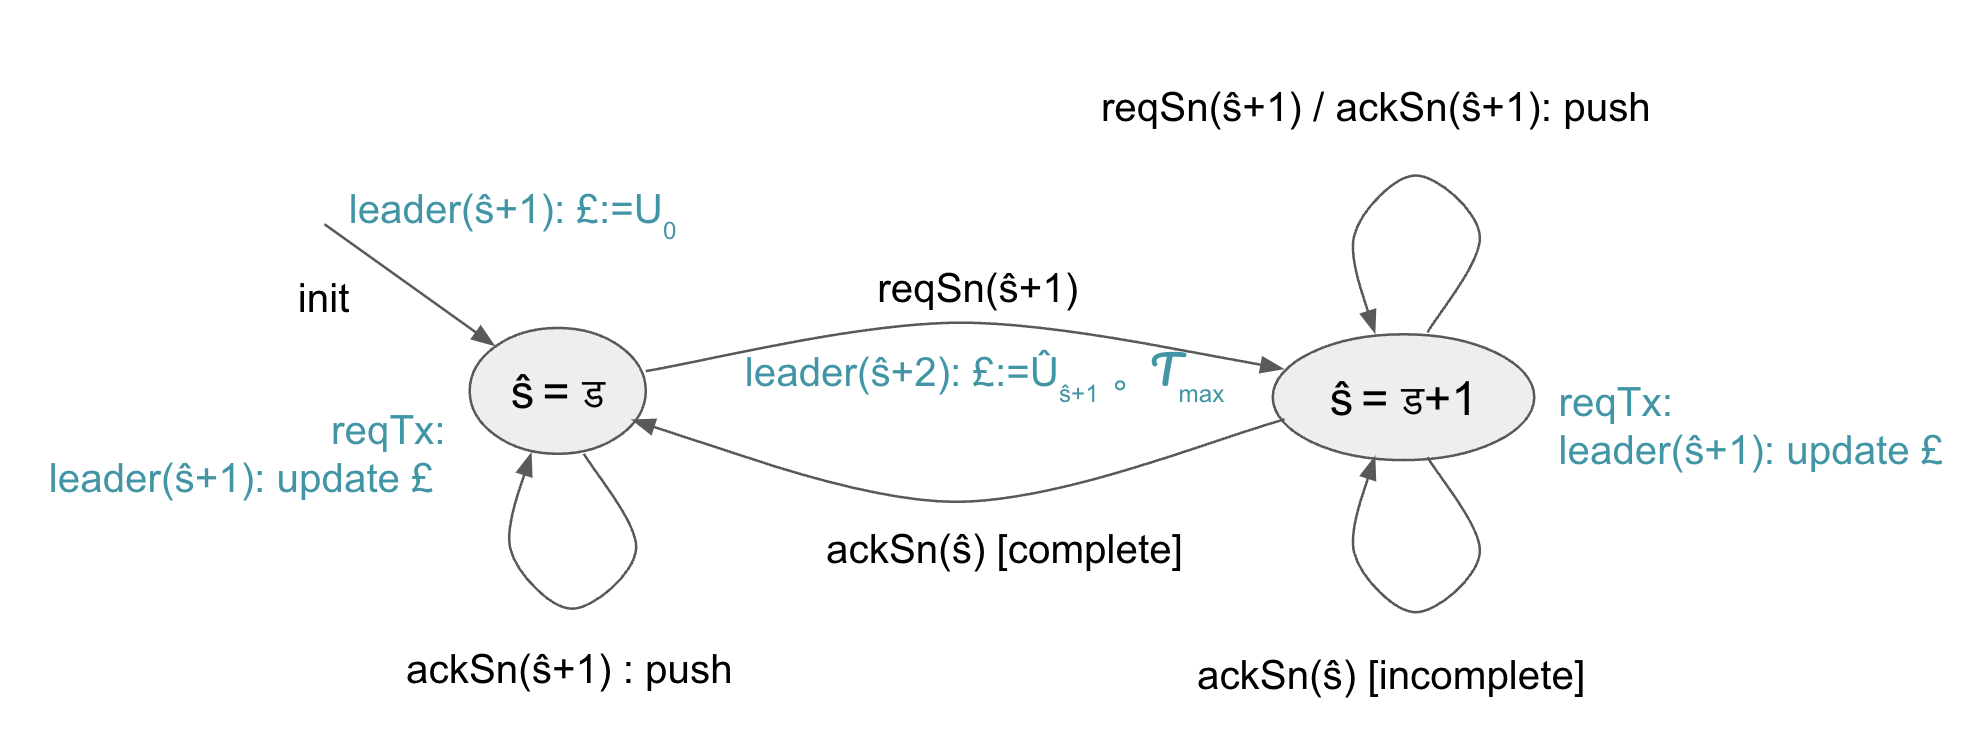
\includegraphics[width=\linewidth*2/3]{fig/reqackstates.png}
                  \caption{State diagram of reqSn/ackSn cycles.}
                  \label{fig:sim:baselines}
\end{figure}



\section{Security (WIP --- Iteration 1)}\label{sec:security}

\todo{Add security experiment}
\noindent Adversaries:

\begin{mdescription}
\item[Active Adversary.] An \emph{active adversary} $\adv$ has full control
  over the protocol, i.e., he is fully unrestricted in the above security game.

 \item[Network Adversary.] A \emph{network adversary} $\adv_\emptyset$ does not corrupt
   any head parties, eventually delivers all sent network messages
   (i.e., does not drop any messages), and does not cause the $\hpClose$ event.
   Apart from this restriction, the adversary can act arbitrarily in the above experiment.
\end{mdescription}

\noindent Random variables:

\begin{mitemize}
\item $\That_i$: the set of transactions $\tx$ for which party $\party_i$,
  \emph{while uncorrupted}, output $(\hpSeen,\tx)$;

\item $\Tbar_i$: the set of transactions $\tx$ for which party $\party_i$,
  \emph{while uncorrupted}, output $(\hpConf,\tx)$;
    
\item $\Snapbar_i$: latest snapshot $(s,U)$ that party
  $\party_i$ performed \emph{while uncorrupted}: output $(\hpSnap,(s,U))$;

\item $\Hcont$: the set of (at the time) uncorrupted parties who produced
  $\xi$ upon close/contest request and $\xi$ was applied to
  correct~$\eta$; and

\item $\honest$: the set of parties that remain uncorrupted.
\end{mitemize}


\noindent Security conditions / events:

\begin{itemize}
\item \propName{Consistency (Head)}: In presence of an active adversary, the
  following condition holds at any point in time:
   For all $i,j$,
   $\Uinit \circ (\Tbar_i \cup \Tbar_j) \not= \bot$, i.e., no two
   uncorrupted parties see conflicting transactions confirmed.

  \item \propName{Oblivious Liveness (Head)}:
    Consider any protocol execution in presence of a network adversary wherein
    the head does not get closed for a sufficiently long period of time, and consider
    an honest party $p_i$ who enters transaction $\tx$ by executing $(\hpNew,\tx)$ \emph{each time after having finished a snapshot}.

    Then the following eventually holds:
    $\tx \in \bigcap_{i\in[n]} \Tbar_i\ \vee\ %
    \forall i: \Uinit \circ (\Tbar_i\cup\{\tx\}) = \bot$,
    i.e., every party will observe the transaction confirmed or every party
    will observe the transaction in conflict with their confirmed transactions.\footnote{
      In particular, \emph{liveness} expresses that the protocol makes progress
      under reasonable network conditions if no head parties get corrupted.
    }

\item \propName{Soundness (Chain)}: In presence of an active adversary,
  the following condition is satisfied:
  $\exists \Ttilde \subseteq \bigcap_{i \in \honest} \That_i : \Ufinal
  = \Uinit \circ \Ttilde\not=\bot$, i.e., the final UTxO set results
  from applying a set of transactions to $U_0$ that have been seen by
  all honest parties (wheras each such transaction applies conforming to the ledger rules).
\item \propName{Completeness (Chain)}: In presence of an active adversary,
  the following condition holds: For $\Ttilde$ as above,
  $\bigcup_{p_i \in \Hcont} \Tbar_i \subseteq \Ttilde$, i.e., all
  transactions seen as confirmed by an honest party at the end of the
  protocol are considered.
\end{itemize}

Note that the original version of the coordinated head satisfies a stronger version of liveness which is important for the 'user experience' in the protocol:
\begin{itemize}
  \item \propName{Liveness (Head)}:
    Consider any protocol execution in presence of a network adversary wherein
    the head does not get closed for a sufficiently long period of time, and consider
    an honest party $p_i$ who enters transaction $\tx$ by executing $(\hpNew,\tx)$.

    Then the following eventually holds:
    $\tx \in \bigcap_{i\in[n]} \Tbar_i\ \vee\ %
    \forall i: \Uinit \circ (\Tbar_i\cup\{\tx\}) = \bot$,
    i.e., every party will observe the transaction confirmed or every party
    will observe the transaction in conflict with their confirmed transactions.\footnote{
      In particular, \emph{liveness} expresses that the protocol makes progress
      under reasonable network conditions if no head parties get corrupted.
    }
\end{itemize}


\subsection{Proofs}

\paragraph{Consistency.}

\begin{lemma}[Consistency]
  \label{lem:consistency}
  The coordinated head protocol satisfies the \propName{Consistency} property.
\end{lemma}
\begin{proof}
  Observe that $\Tbar_i\cup\Tbar_j\subseteq\That_i$ since no
  transaction can be confirmed without every honest party signing off
  on it.  Since parties do not sign conflicting transactions
  (see $\hpRS$, `wait'), we have
  $\Uinit\applytx\Tbar_i\neq\bot$,
  $\Uinit\applytx\Tbar_j\neq\bot$, and
  $\Uinit\applytx\That_i\neq\bot$.  Thus, since $\Tbar_i\cup\Tbar_j\subseteq\That_i$
  it follows that
  $\Uinit\applytx(\Tbar_i\cup\Tbar_j)\neq\bot$
\end{proof}

\paragraph{Oblivious Liveness.}
For all lemmas towards oblivious liveness, we assume the presence of a network adversary, and that the head does not get closed for a sufficiently
long period of time.
We call this the \emph{liveness condition}.

\begin{lemma}\label{lem:reqconf}  
  Under the liveness condition, any snapshot issued as $(\hpRS,s,T)$ will eventually be confirmed
  in the sense that every party holds a valid mulisignature on it.
\end{lemma}
\begin{proof}
  Consider a party $p_i$ receiving message $(\hpRS,s,T)$. We demonstrate that $p_i$ executes
  the code past the `wait' instruction of the $\hpRS$ routine. 

  \begin{itemize}
   \item Passing the `require' guard:
  Note that the snapshot leader sends the request only if $\hats=\bars$, and for $s=\hats+1$.
  Thus, $\hats_i=\hats$ since $p_i$ has already signed the snapshot for $\hats$. The `require'
  guard is thus satisfied for $p_i$.

   \item Passing the `wait' guard:
  Since the snapshot leader sees $\hats=\bars$, also $p_i$ will eventually see $\hats_i=\bars_i$. Furthermore, since all leaders are honest, it holds that $\hatmU\applytx\mT_{res}\not=\bot$ by construction.
  \end{itemize}

  This implies that every party will eventually sign and acknowledge the newly created snapshot.
  Finally, the `require' and `wait' guards of the $\hpAS$ code will be passed by every party
  since an $\hpAS$ for snapshot number $s$ can only be received for $s\in\{\hats,\hats+1\}$
  as an acknowledgement can only be received for the current snapshot being worked on by $p_i$
  or a snapshot that is one step ahead---implying that everybody will hold a valid multisignature
  on the snapshot in consideration.
\end{proof}

\begin{lemma}[Eternal snapshot confirmation]\label{lem:eternal}
  Under the liveness condition, as long as new transactions are issued, for any $k>0$, every party eventually confirms
  a snapshot with sequence number $s=k$.
\end{lemma}
\begin{proof}
  By Lemma~\ref{lem:reqconf}, any requested snapshot eventually gets confirmed, implying
  that the next leader observes $\hats=\bars$ and thus, in turn, issues a new snapshot.
  Thus, for any $k$, a snapshot is eventually confirmed.
\end{proof}

\begin{lemma}[Oblivious Liveness]
  \label{lem:liveness}
  The coordinated head protocol satisfies the \propName{Oblivious Liveness} property.
\end{lemma}
\begin{proof}
  Consider the first point in time where a transaction $\tx$ enters the system by some party $p_i$
  issuing $(\hpNew,\tx)$, and consider the next point in time
  $t$ when $p_i$ issues a snapshot.

  By Lemma~\ref{lem:eternal}, this snapshot will eventually be issued and confirmed by all parties.
  
  \medskip
  
  Let $\hatmT$ be the transactions to be considered by $p_i$'s snapshot: $\hatmL=\barmU\applytx\hatmT$
  where $\barmU$ is the snapshot prior to $p_i$'s. Since $p_i$ issues
  $(\hpRT,\tx)$ after each snapshot, we have that, either,
  \begin{itemize}
      \item $\tx\in\hatmT$, in which case $\tx \in \bigcap_{i\in[n]} \Tbar_i$ after everybody has completed this snapshot, or,
      \item $\tx\notin\hatmT$, in which case $\hatmL\applytx\tx=\bot$ ($\tx$ is still in the wait queue of $(\hpRT,\tx)$. After everybody has completed this snapshot, it thus holds that $\forall i: \Uinit\applytx\bigcap_{i\in[n]}{\Tbar_i}=\hatmL$, and .
  \end{itemize}
  In both cases, the lemma follows.
\end{proof}

\paragraph{Soundness and completeness.}

\begin{lemma}[Soundness]
  \label{lem:soundness}
  The basic head protocol satisfies the \propName{Soundness} property.
\end{lemma}

\begin{proof}
  Let $T$ be the set of transactions such that $\Ufinal=U_0\applytx T$.
  Since $\Ufinal$ is multi-signed, it holds that $T\subseteq\That_i$
  ($T$ is \emph{seen}) by every honest party in the head.
  Furtermore, since honest signatures are only issued for valid transaction,
  $\Ufinal\not=\bot$ (i.e., $\Ufinal$ is a valid state), and soundness
  follows.
\end{proof}


\begin{lemma}[Completeness]
 \label{lem:completeness}
 The basic head protocol satisfies the \propName{Completeness}
 property.
\end{lemma}
\begin{proof}
  Consider all parties $p_i\in\Hcont$. Since the close/contest process
  finally accepts the latest multi-signed snapshot, it holds that
  $\Ufinal.s \geq \max_{p_i\in\Hcont}(\bars_i)$, and thus that
  $\bigcup_{p_i\in\Hcont}\Tbar_i\subseteq\bigcap_{p_i\in\honest}\That_i$,
  and completeness follows.
\end{proof}

%%% Local Variables:
%%% mode: latex
%%% TeX-master: "main"
%%% End:


\bibliographystyle{plain}
\bibliography{short}

\end{document}
